\chapter{Time Series}

\section{Model Selecting}

\begin{itemize}
\item to find a model with the smallest out-of-the-sample 1-ahead mean squared prediction error
\item mean squared error - corresponds to selecting a model with the highest $R^2$; does not penalize for number of predictive variables $\Rightarrow$ in-sample overfitting
\begin{equation*}
MSE = \frac{\sum_{t=1}^T}{T}
\end{equation*}
\item MSE corrected for degrees of freedom - corresponds to selecting a model with the highest $\overline{R^2}$
\begin{equation*}
s^2 = \frac{T}{T - k} MSE
\end{equation*}
\item Akaike information criterion - heavier penalization for degrees of freedom than $s^2$
\begin{equation*}
AIC = e^{\frac{2k}{T}}MSE
\end{equation*}
\item Schwarz information criterion - heavier penalization for degrees of freedom than AIC
\begin{equation*}
SIC = T^{\frac{k}{T}}MSE
\end{equation*}
\item the lower the selection criterion the better
\item consistency - probability of the true DGP (or DGP closest to the true DGP) selection increases with sample size
\item effectivness - DGP 1-step-ahead forcast error variances approach the one that would be obtained using the true DGP with increasing sample size
\item SIC is consistent but not efficient; AIC is efficient but not consistent
\item if SIC and AIC select different DGP, we prefer SIC over AIC
\end{itemize}

\begin{figure}[htp]
\centering
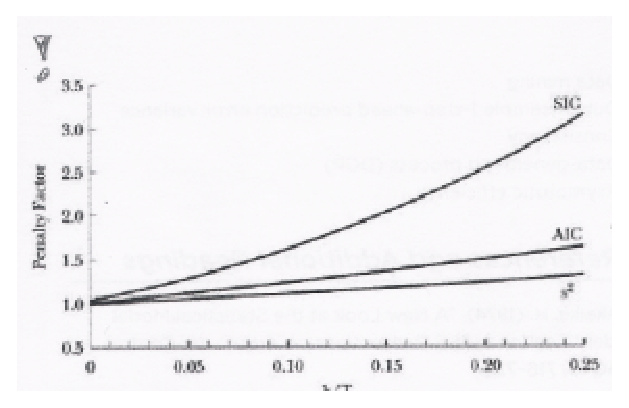
\includegraphics[scale = 0.75]{selection_criterion.eps}
\caption{$s^2$, AIC and SIC "punishment" for number of degrees of freedom}
\label{selection_criterion}
\end{figure}

\section{Characterizing Cycles}

\begin{itemize}
\item covariance stationarity - necesary if we want to predict time series
\begin{itemize}
\item mean - $E[y_t] = \mu$
\item autocovariance - $\gamma(t, \tau) = cov(y_t, y_{t-\tau}) = \gamma(\tau)$
\begin{gather*}
\gamma(\tau) = \gamma(-\tau)\\
\gamma(0) = cov(y_t, y_t) = D[y_t]\\
0 < \gamma(0) < \infty
\end{gather*}
\end{itemize}
\item many economic time series is not stationary but can be converted to stationary ones - from absolute to relative changes, remove seasonalities and trends
\item autocorerlation function - ordinary correlation between $y_t$ and $y_{t-\tau}$
\begin{equation*}
\rho(\tau) = \frac{\gamma(\tau)}{\gamma(0)}
\end{equation*}
\item partial autocorerlation function - correlation between $y_t$ and $y_{t-\tau}$ with other $y_{t-i}$ being constant $\Rightarrow$ coeficient of autoregression function
\begin{equation*}
\rho(\tau) = \frac{\gamma(\tau)}{\gamma(0)}
\end{equation*}
\item white noise
\begin{equation*}
y_t = \epsilon_t ~~~ \epsilon_t \sim (0, \sigma^2)
\end{equation*}
\begin{itemize}
\item shock $\epsilon_t$ is serially uncorellated $Rightarrow$ serially uncorrelated white noise
\item if shock $\epsilon_t$ is normally distributed $Rightarrow$ independent white noise
\item autocovariance $\gamma(0) = \sigma^2 ~~~ \gamma(\tau \ge 0) = 0$
\item autocorrelation $\rho(0) = 1 ~~~ \rho(\tau \ge 0) = 0$
\item partial autocorrelation $p(0) = 1 ~~~ p(\tau \ge 0) = 0$
\item uncoditional mean and variance are constant by covariance stationarity vs. conditional mean and variance
\end{itemize}
\item lag operator
\begin{gather*}
L y_t = y_{t-1}\\
L^m y_t = y_{t-m}\\
B(L) y_t = b_0 + b_1L + b_2L^2 + ...\\
B(L)\epsilon_y = b_0 \epsilon_t + b_1 \epsilon_{t-1} + b_2 \epsilon_{t-2} + ... = \sum_{i = 0}^{\infty} b_i \epsilon_{t-i}
\end{gather*}
\item Wold's theorem - any zero-mean covariance-stationary process can be written as
\begin{equation*}
y_t = B(L)\epsilon_t = \sum_{i = 0} ^ {\infty} b_i \epsilon_{t-i} ~~~b_0 = 1, \sum_{i = 0}^{\infty} b_i^2 < \infty
\end{equation*}
\begin{itemize}
\item the above is called general linear process
\item shock $\epsilon_t$ is serially uncorrelated but not necessarily independent
\item if a covariance stationary series $y_t$ has mean of $\mu$ we define $y_t^* = y_t - \mu$
\item unconditional moments - stable in time
\begin{gather*}
E[y_t] = E\left[\sum_{i = 0}^{\infty} b_i \epsilon_{t-i}\right] = 0\\
D[y_t] = D\left[\sum_{i = 0}^{\infty} b_i \epsilon_{t-i}\right] = \sigma^2 \sum_{i = 0}^{\infty}b_i^2
\end{gather*}
\item conditional moments - move over time in response to the evolving information set
\begin{gather*}
E[y_t|\Omega_{t-1}]= E\left[\sum_{i = 0}^{\infty} b_i \epsilon_{t-i} | \Omega_{t-1}\right] = \sum_{i = 1}^{\infty} b_i \epsilon_{t-i}\\
D[y_t|\Omega_{t-1}]= D\left[\sum_{i = 0}^{\infty} b_i \epsilon_{t-i} | \Omega_{t-1}\right] = b_0 \sigma^2 = \sigma^2
\end{gather*}
\item infinite order polynomial $B(L)$ (and therefore Wold's theorem as well) can be approximated by rational polynomials
\begin{equation*}
B(L)  \approx \frac{\Theta(L)}{\Phi(L)} = \frac{\sum_{i = 0}^p \theta_i L^i}{\sum_{i = 0}^q \phi_i L^i}
\end{equation*}
\item sample autocorrelation
\begin{itemize}
\item sample mean
\begin{equation*}
\overline{y} = \frac{1}{T}\sum_{t = 1}^T y_t
\end{equation*}
\item sample autocorrelation
\begin{equation*}
\hat{\rho}(\tau) = \frac{\frac{1}{T}\sum_{t = \tau + 1}^T\left(y_t - \overline{y})(y_{t - \tau} - \overline{y})\right)}{\frac{1}{T}\sum_{t=1}^T(y_t - \overline{y})^2}
\end{equation*}
\item if a particular autocorrelation $\hat{\rho}(\tau)$ is 0, then
\begin{equation*}
\hat{\rho}(\tau) \sim N\left(0, 1/T \right)
\end{equation*}
\item if all autocorrelations are 0, then
\begin{gather*}
T\hat{\rho}^2(\tau) \sim \chi_1^2\\
T \sum_{\tau = 1}^m \hat{\rho}^2(\tau) \sim \chi_m^2
\end{gather*}
\item Box-Pierce Q-statistics $Q_{BP} = T \sum_{\tau = 1}^m \hat{\rho}^2(\tau)$
\item Ljung-Box Q-statistics $Q_{LB} = T (T + 2)\sum_{\tau = 1}^m \left(\frac{1}{T - \tau} \right)\hat{\rho}^2(\tau)$
\item $m$ is usually selected in neighbordhood of $\sqrt{T}$
\end{itemize}
\item sample partial autocorrelation - if the series is white noise, approximately 95\% of the sample partial autocorrelations should fall in the intereval $\pm 2 / \sqrt{T}$
\begin{gather*}
\hat{y}_t = \hat{c} + \hat{\beta}_1 y_{t - 1} + ... + \hat{\beta}_{\tau} y_{t - \tau}\\
\hat{p}(\tau) \equiv \hat{\beta}_{\tau}
\end{gather*}
\item correlogram analysis - plot autocorrelations and partial autocorrelations for individual displacements $\Rightarrow$ tells with type process is the most sutaible
\end{itemize}
\begin{figure}[htp]
\centering
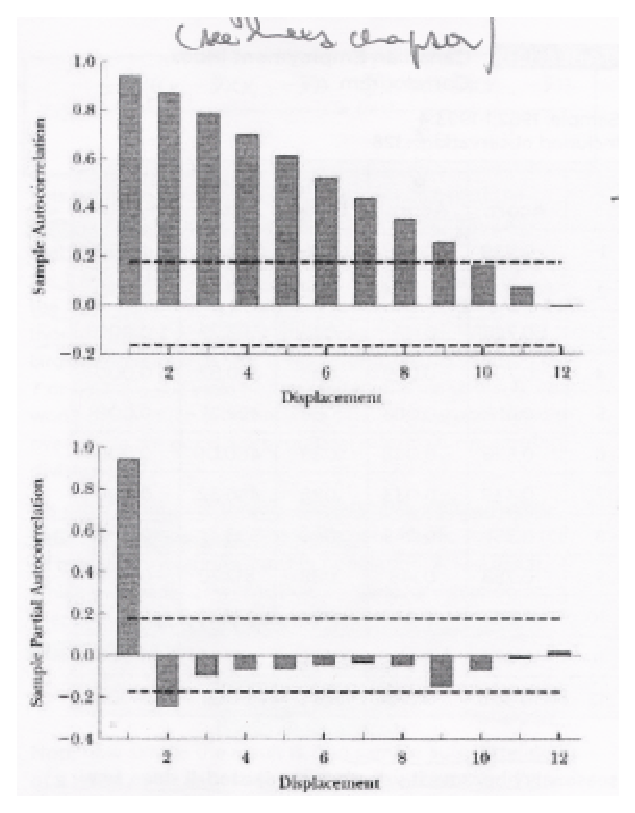
\includegraphics[scale = 0.75]{correlogram.eps}
\caption{correlogram for autocorrelation and partial autocorrelation function}
\label{correlogram}
\end{figure}
\end{itemize}

\section{MA, AR and ARMA Models}

\subsection{MA Models}

\subsubsection{MA(1) Model}

\begin{itemize}
\item MA(1): $y_t = \epsilon_t + \theta \epsilon_{t-1} = (1 + \theta L)\epsilon_t$ where $\epsilon_t$ is zero-mean white noise (not necessarily normaly distributed)
\item always covariance stationary but not always invertible (requires $|\theta| < 1$)
\item autocorrelation function was cut-off beyond $\tau > 0$
\item partical autocorrelation function is oscilating
\item unconditional moments
\begin{gather*}
E[y_t] = E[\epsilon_t] + \theta[\epsilon_{t - 1}] = 0\\
D[y_t] = D[\epsilon_t] + \theta^2 D[\epsilon_{t - 1}] = (1 + \theta^2)\sigma^2
\end{gather*}
\item conditional moments
\begin{gather*}
E[y_t | \Omega_{t-1}] = E[\epsilon_t | \Omega_{t-1}] + \theta[\epsilon_{t - 1} | \Omega_{t-1}] = \theta \epsilon_{t - 1}\\
D[y_t | \Omega_{t-1}] = D[\epsilon_t | \Omega_{t-1}] + \theta^2 D[\epsilon_{t - 1}| \Omega_{t-1}] = \sigma^2
\end{gather*}
\item autocorrelation function $\gamma(0) = \theta \sigma^2 ~~~ \gamma(\theta > 0) = 0$
\item MA(1) is invertible is $|\theta| < 1$ $\Rightarrow$ MA(1) can be expressed in autoregressive form (the below sum converge)
\begin{gather*}
y_t = \epsilon_t + \theta \epsilon_{t - 1}\\
\epsilon_{t - 1} = y_{t - 1} - \theta \epsilon_{t - 2}\\
y_t = \epsilon_t + \theta y_{t-1} - \theta^2 y_{t-2} + \theta^3 y_{t - 3} - ...
\end{gather*}
\end{itemize}

\begin{figure}[htp]
\centering
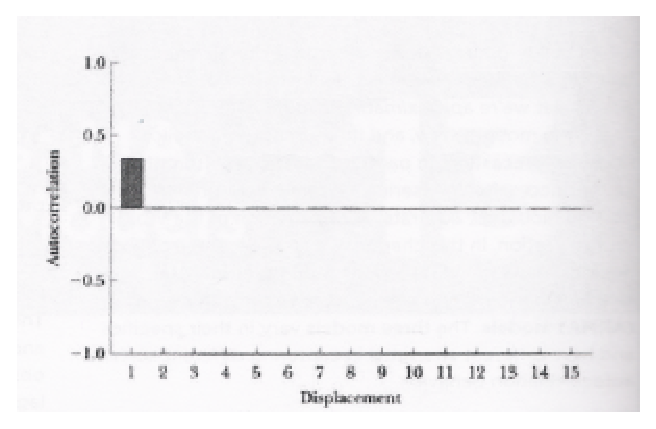
\includegraphics[scale = 0.75]{MA1.eps}
\caption{MA(1) - correlogram of autocorrelation function}
\label{MA1}
\end{figure}

\begin{figure}[htp]
\centering
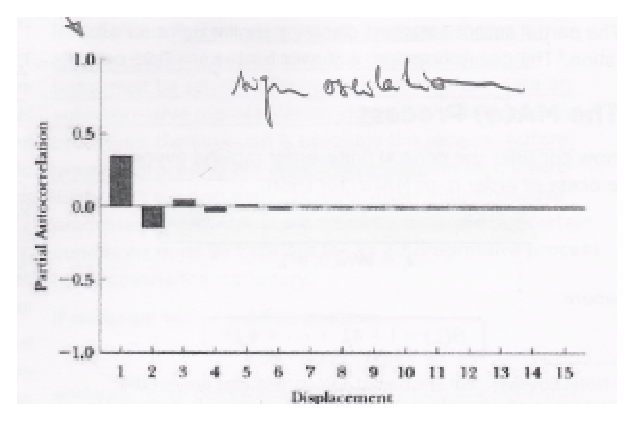
\includegraphics[scale = 0.75]{MA2.eps}
\caption{MA(1) - correlogram of partial autocorrelation function}
\label{MA2}
\end{figure}

\subsubsection{MA(q) Model}

\begin{itemize}
\item MA(q): $y_t = \epsilon_t + \theta_1 \epsilon_{t-1} + ... + \theta_q \epsilon_{t - q} = \Theta(L)\epsilon_t$ where $\epsilon_t$ is zero-mean white noise (not necessarily normaly distributed)
\item autocorrelation function cut-off is at displacement $q$
\item partial autocorrelation function dacays gradually
\item can capture richer dynamic patterns than MA(1) because of its higher order polynomial
\item is always covariance stationary
\item is invertible only if roots of $\Theta(L)$ are within a unit circle
\end{itemize}

\subsection{AR Models}

\subsubsection{AR(1) Model}

\begin{itemize}
\item AR(1): $y_t = \varphi y_{t - 1} + \epsilon_{t} \Leftrightarrow (1 - \varphi L)y_t = \epsilon_t$ where $\epsilon_t$ is zero-mean white noise (not necessarily normaly distributed)
\item always invertible but not always covariance stationary (requires $|\varphi| < 1$)
\item lag operator in form of
\begin{equation*}
y_t = \frac{1}{1 - \varphi L} \epsilon_t
\end{equation*}
\item special case of MA($\infty$) with $\theta_i = \theta^i$
\begin{equation*}
y_t = \epsilon_t + \varphi \epsilon_{t-1} + \varphi^2 \epsilon_{t-2} + ...
\end{equation*}
\item autocorrelation function decays gradually
\item partial autocorrelation functions has cut-off at displacement 0 
\item fluctuation is much more persistent than in case of MA(1) $\Rightarrow$ able to capture much more persistent dynamics than MA(1)
\item unconditional moments
\begin{gather*}
E[y_t] = E[\epsilon_t + \varphi \epsilon_{t-1} + \varphi^2 \epsilon_{t-2} + ...] = 0\\
D[y_t] = D[\epsilon_t + \varphi \epsilon_{t-1} + \varphi^2 \epsilon_{t-2} + ...] = \frac{1}{1 - \varphi^2}\sigma^2
\end{gather*}
\item conditional moments
\begin{gather*}
E[y_t | \Omega_{t - 1}] = E[\varphi y_{t - 1} + \epsilon_{t} | \Omega_{t - 1}] = \varphi y_{t - 1}\\
D[y_t | \Omega_{t - 1}] = D[\varphi y_{t - 1} + \epsilon_{t} | \Omega_{t - 1}] = \sigma^2
\end{gather*}
\item covariance function - Yule-Walker equation
\begin{gather*}
y_t y_{t - \tau} = \varphi y_{t - 1} y_{t - \tau} + \epsilon y_{t - \tau}\\
E[y_t y_{t - \tau}] = E[\varphi y_{t - 1} y_{t - \tau} + \epsilon y_{t - \tau}]\\
\gamma(\tau) = \varphi \gamma (\tau - 1)\\
\gamma(\tau) = \varphi^{\tau} \frac{\sigma^2}{1 - \varphi^2}
\end{gather*}
\item autocorrelation function $\rho(\tau) = \varphi^{\tau}$ $\Rightarrow$ autocorrelation function decays gradually; if $\varphi > 0$ the decay is one-sided
\item partial autocorrelation function $p(1) = \varphi ~~~ p(\tau > 1) = 0$
\end{itemize}

\begin{figure}[htp]
\centering
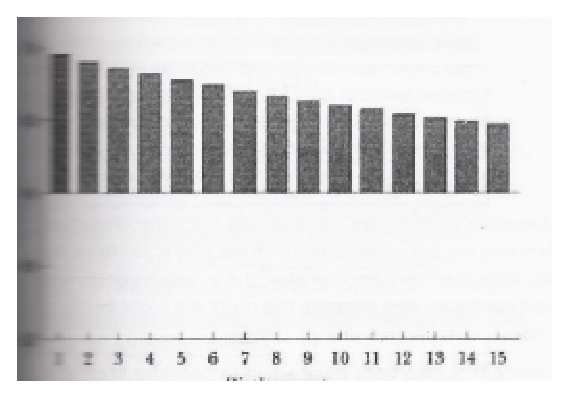
\includegraphics[scale = 0.75]{AR1.eps}
\caption{AR(1) - correlogram of autocorrelation function}
\label{AR1}
\end{figure}

\begin{figure}[htp]
\centering
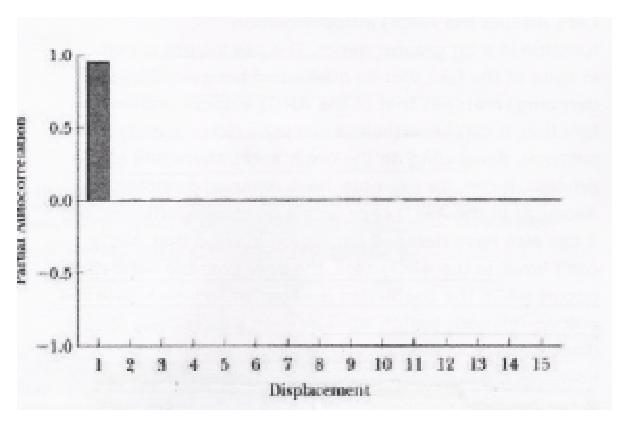
\includegraphics[scale = 0.75]{AR2.eps}
\caption{AR(1) - correlogram of partial autocorrelation function}
\label{AR2}
\end{figure}


\subsubsection{AR(q) Model}

\begin{itemize}
\item AR(q): $y_t = \varphi_1 y_{t-1} + \varphi_2 y_{t-2} + ... + \varphi_q y_{t-q} + \epsilon_t \Leftrightarrow \epsilon_t = \Phi(L)y_t$ where $\epsilon_t$ is zero-mean white noise (not necessarily normaly distributed)
\item autocorrelation function decays gradually (may oscilate)
\item partial autocorrelation function has a cut-off at displacement $q$
\item is always invertible
\item is invertible only if roots of $\Phi(L)$ are withing a unit circle
\end{itemize}

\subsection{ARMA Models}

\begin{itemize}
\item neither autocorrelation nor partial autocorrelation functions have a cut-off
\item more accurate approximation of Wold's theorem than MA or AR processes with the same number of parameters
\item ARMA models creation
\begin{itemize}
\item combining MA and AR models
\item random shock ifself is a moving average
\item AR processes subject to measurement error also turn out to be ARMA processes
\end{itemize}
\item ARMA(1,1): $y_t = \varphi y_1 + \epsilon_t + \theta \epsilon_{t - 1} \Leftrightarrow (1 - \varphi)L y_t = (1 + \theta L)\epsilon_t$
\begin{itemize}
\item is invertible if $|\theta| < 1$ $\Rightarrow$ $\epsilon_t = \frac{1 - \varphi L}{1 + \theta L} y_t$
\item is covariance stationary if $|\varphi| < 1$ $\Rightarrow$ $y_t = \frac{1 + \theta L}{1 - \varphi L} \epsilon_t$
\end{itemize}
\item ARMA(p,q): $y_t = \varphi_1 y_{t-1} + ... + \varphi_p y_{t - p} + \epsilon_t + \theta_1 \epsilon_{t - 1} + ... + \theta_q \epsilon_{t - q} \Leftrightarrow \Theta(L)y_t = \Phi(L) \epsilon_t$
\begin{itemize}
\item is invertible if inverses of all roots of $\Theta(L)$ are within a unit circle $\Rightarrow$ $y_t = \frac{\Theta(L)}{\Phi(L)}\epsilon_t$
\item is covariance stationary if inverses of all roots of $\Phi(L)$ are within a unit circle $\Rightarrow$ $\epsilon_t = \frac{\Phi(L)}{\Theta(L)}y_t$
\end{itemize}
\end{itemize}

\subsection{Application}

\begin{itemize}
\item select model with the lowest SIC / AIC
\item plot collerogram for autocorrelation and partial autocorrelation function
\end{itemize}

\subsubsection{MA Processes}

\begin{itemize}
\item non-linear in parameters $\Rightarrow$ parameter estimation using numerical minimalization
\begin{gather*}
y_t = \epsilon_t + \theta \epsilon_{t - 1}\\
\hat{y}_t \approx \theta y_{t-1} - \theta^2 y_{t - 2} + ... + (-1)^{m + 1} \theta ^ m y_{t - m} + \epsilon_t
\end{gather*}
\item try to find $\theta$ that minimizes $\sum_{t = 1}^T (\hat{y}_t - y_t)^2$
\item if the model fits the underlying process $(\hat{y}_t - y_t)$ is a white noise
\end{itemize}

\subsubsection{AR Processes}

\begin{itemize}
\item parameters could be easily estimated through linear regression
\begin{equation*}
y_t = \varphi y_{t - 1} + \epsilon_t
\end{equation*}
\end{itemize}

\subsubsection{ARMA Processes}

\begin{itemize}
\item parameter estimation is similar to MA models
\item AR(2) vs ARMA(3,1) and common factors - arises when $\varphi_i = \theta_i$
\begin{gather*}
ARMA(0, 0): ~ y_t = \epsilon_t\\
ARMA(1, 1): ~ y_t - \alpha y_{t - 1} = \epsilon_t - \alpha \epsilon_{t - 1} \Rightarrow y_t = \alpha y_{t - 1} + \epsilon_t - \alpha \epsilon_{t - 1}
\end{gather*}
\end{itemize}
